\appendix \label{sec:app}
\section{Detailed Barycentric Interpolation Methods}
\subsection{Triangulating a \glsentrytitlecase{vfz}{long} Mesh}
\label{app:bary-tri}

% Briefly (but clearly and explicitly) explain the steps of generating the cubochorically sampled GBs, converting them to octonions and then mapping all of them into the vfz. Then explain how you do the triangulation. This will require a few figures to show the process in 3D (i.e. generating a triangulation of a point cloud on a region of the surface of the 2-sphere).

% After random \glspl{vfzo} are obtained (\cref{sec:methods:rand}), % ...

In order to reduce the computational complexity of triangulating a high-dimensional mesh \cite{barberQuickhullAlgorithmConvex1996}, some simplifications are made. The degenerate dimension obtained from analytically minimizing $U(1)$ symmetry \cite{francisGeodesicOctonionMetric2019} is first removed via a rigid (i.e. distance- and angle-preserving) \gls{svd} transformation,
%to enable use of MATLAB's quickhull \cite{barberQuickhullAlgorithmConvex1996} implementations such as \texttt{delaunayn} and \texttt{convhulln}. Removal of the degenerate dimension is done via a rigid \gls{svd} transformation,
analogous to a Cartesian rotation and translation
%Thus, a set of octonions originally represented by 8D Cartesian coordinates are collapsed to a 7D Cartesian representation while preserving both distances and angles among the points
As a 3D Cartesian to 2D Cartesian analogue of this 8D Cartesian to 7D Cartesian transformation, we take a set . Next, this 7D Cartesian representation is projected onto a hyperplane tangent to the mean of the input points\footnote{This is \textit{not} a rigid transformation; however, it is sufficiently close to produce a high-quality triangulation in a \gls{vfz}.} (\cref{fig:bary-delaunay}b). The 7D Cartesian \glspl{gbo} undergo another rigid \gls{svd} transformation to 6D Cartesian (see 3D to 2D analogue in \cref{fig:bary-delaunay}c) for which a triangulation is computed via the quickhull algorithm \cite{barberQuickhullAlgorithmConvex1996} (see MATLAB function \texttt{delaunayn}).

\begin{figure}
    \centering
    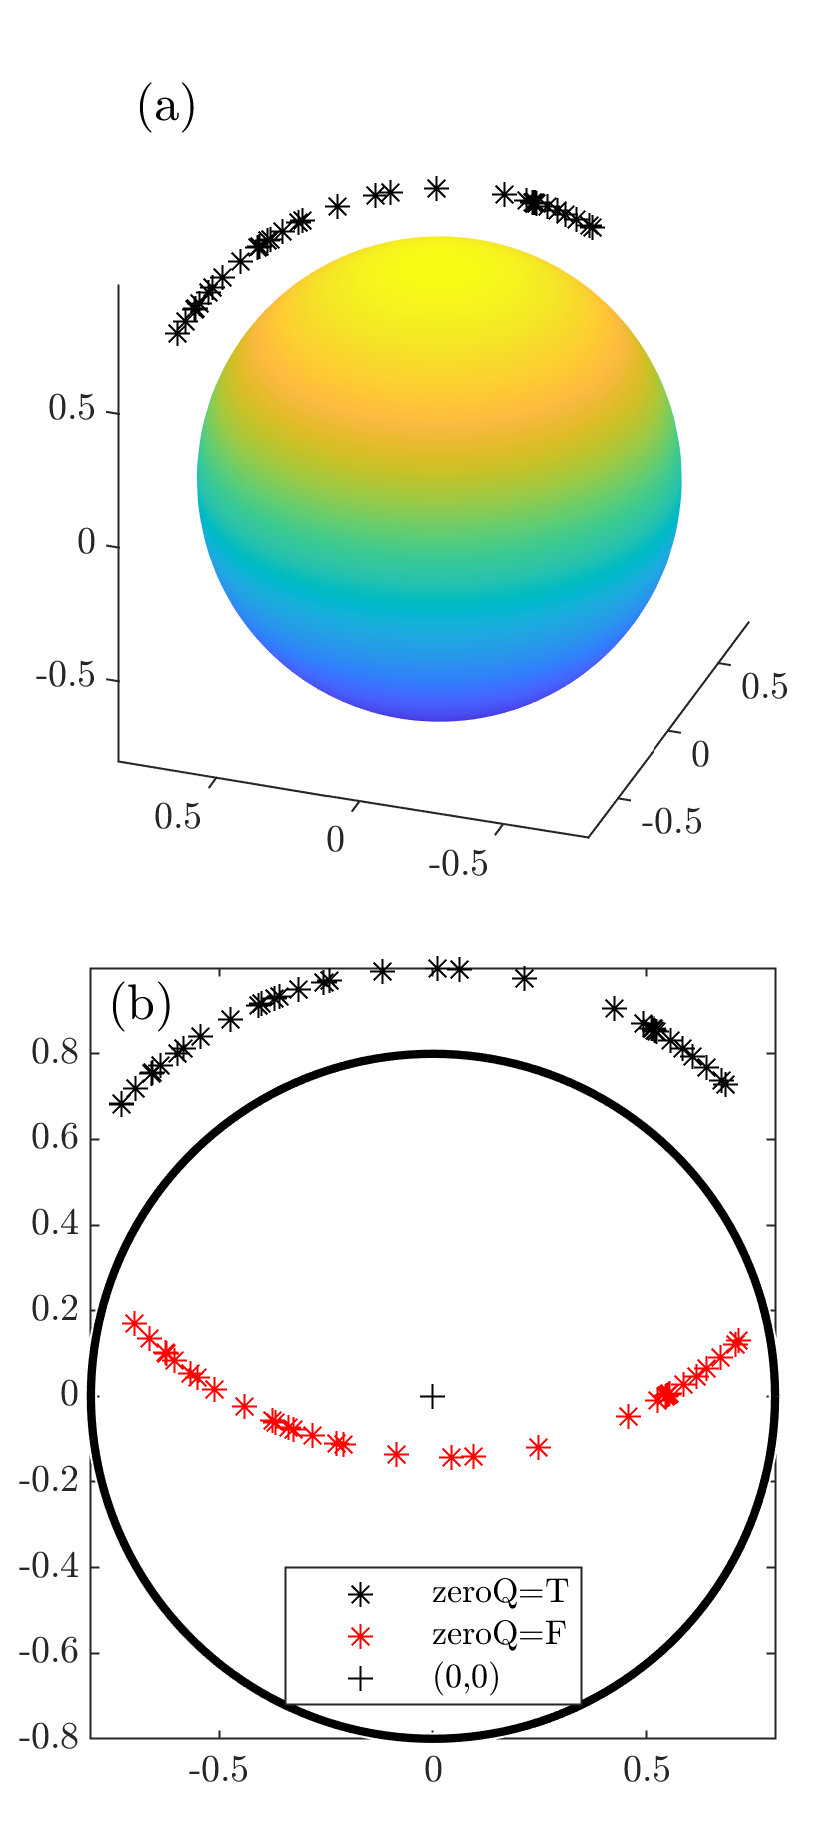
\includegraphics[scale=1]{bary-remove-deg.png}
    \caption{3D Cartesian to 2D Cartesian analogue of 8D Cartesian to 7D Cartesian degeneracy removal used in barycentric interpolation approach. Starting spherical arc points on surface of 2-sphere (a) and degenerate dimension removed via \acrlong{svd} transformation to 2D Cartesian (b) with either the origin (black plus) preserved (black asterisks, \texttt{zeroQ=T}) or ignored (red asterisks, \texttt{zeroQ=F}). The sphere (a) and circle (b) each have a radius of 0.8 and are used as a visualization aid only.}
    \label{fig:bary-remove-deg}
\end{figure}

Using a separate rigid \gls{svd} transformation from the triangulation, the original mesh and prediction \glspl{gbo} are simultaneously transformed from 8D Cartesian to 7D Cartesian. Because our \gls{svd} approach is rigid, the triangulation is then superimposed onto the newly transformed input points resulting in a 7D Cartesian \gls{vfz}.

\begin{figure}
    \centering
    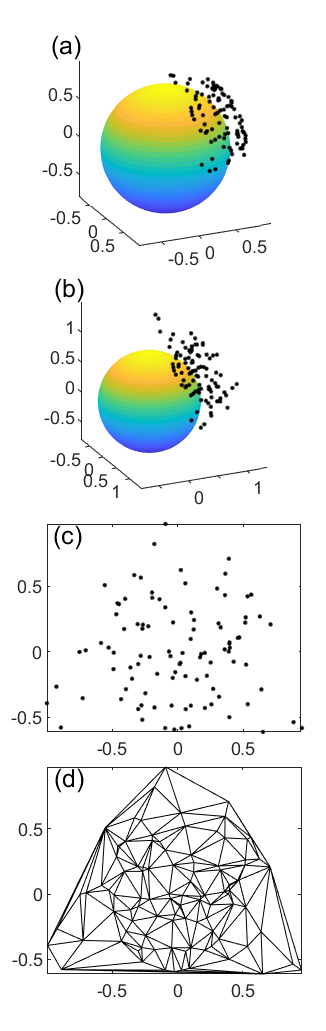
\includegraphics[scale=1]{bary-delaunay.png}
    \caption{3D Cartesian to 2D Cartesian analogue of 7D Cartesian to 6D Cartesian mesh triangulation used in barycentric interpolation approach. Normalized starting points on surface of 2-sphere (a), points projected onto hyperplane tangent to mean of starting points (b), degenerate dimension removed via rigid \gls{svd} transformation to 2D Cartesian (c), and Delaunay triangulation in 2D Cartesian (d). The sphere in (a) and (b) has a radius of 0.8 and is used as a visualization aid only.}
    \label{fig:bary-delaunay}
\end{figure}

% In order to reduce the computationally complexity of computing barycentric coordinates in a high-dimensional space \cite{barberQuickhullAlgorithmConvex1996}, a single degenerate dimension (originally introduced by analytically minimizing $U(1)$ symmetry) is removed to enable use of MATLAB's quickhull \cite{barberQuickhullAlgorithmConvex1996} implementations such as \texttt{delaunayn} and \texttt{convhulln}. Removal of the degenerate dimension is done via a rigid \gls{svd} transformation, analogous to a Cartesian rotation and translation. Thus, a set of octonions originally represented by 8D Cartesian coordinates are collapsed to a 7D Cartesian representation while preserving both distances and angles among the points (see 3D to 2D analogue in \cref{fig:bary-remove-deg}). To further reduce the "curse of dimensionality" in computing the triangulation, a 7D Cartesian representation of the octonions constrained to lie on the surface of the 6-sphere are first projected onto a hyperplane tangent to the mean of the input points and then rotated/translated again via \gls{svd} to produce a 6D Cartesian representation (see 3D to 2D analogue in Figure \cref{fig:bary-delaunay}). This 6D representation is used to compute a triangulation via the built-in MATLAB routine \texttt{delaunayn} based on the quickhull algorithm \cite{barberQuickhullAlgorithmConvex1996}, giving facet vertices for the 7D Cartesian hypersphere.

\subsection{Intersections in a \glsentrytitlecase{vfz}{long} Mesh}
\label{app:bary-int}
An intersection is calculated by linearly projecting a prediction point onto the hyperplane defined by a mesh facet's vertices, computing barycentric coordinates within the facet, and testing for positivity \cite{langerSphericalBarycentricCoordinates2006}, and repeating this process until an intersection is found or a stop condition is reached (see \texttt{nnMax} below). If the prediction point is contained within the simplex, all of the barycentric weights (i.e. coordinates) are positive. If it outside the simplex, this constraint is violated. Due to the large number of facets per point of a high-dimensional
%simplex-based
triangulation
%and for computational speed,
prediction point intersections are calculated by considering facets connected to up to some number of mesh \glspl{nn} (\texttt{nnMax}) (in this work, \texttt{nnMax = 10}). For prediction points where no intersecting facet is found
%in these connected facets due to high-aspect ratio facets or prediction point falling outside the mesh within a given tolerance,
a \gls{nn} approach is used (\cref{sec:methods:interp:nn}), which represent average non-intersection rates of \SI{0.1207 \pm 1.02}{\percent} and \SI{0.68 \pm 0.11}{\percent} for input meshes of \num{388} and \num{50000}, respectively, for \num{10000} query points out of \num{10} trials.

\subsubsection{Interpolation via Barycentric Coordinates}
\label{app:bary-interp}

Once barycentric coordinates are computed for a prediction point within the input mesh, the interpolated value is found by taking the dot product of the barycentric coordinates and the properties of the corresponding vertices of the intersecting facet via
\begin{equation}
v=\underset{i=1}{\overset{N}{\sum }}\lambda _i v_i
\end{equation}
where $\lambda$, $v$, $v_i$ and $N$, are the barycentric coordinates, interpolated property, property of the $i$th vertex of the intersecting facet, and number of vertices in a given facet ($N = 7$ for the degeneracy-free 6-sphere).